\documentclass[12pt,a4paper]{article}
\usepackage[utf8]{inputenc}
\usepackage[T1]{fontenc}
\usepackage[spanish]{babel}
\usepackage{geometry}
\usepackage{graphicx}
\usepackage{xcolor}
\usepackage{hyperref}
\usepackage{booktabs}
\usepackage{array}
\usepackage{enumitem}
\usepackage{listings}
\usepackage{tcolorbox}
\usepackage{float}
\geometry{margin=2.5cm}

\hypersetup{
  colorlinks=true,
  linkcolor=black,
  urlcolor=blue,
  citecolor=black
}

\lstdefinestyle{pyclean}{
  language=Python,
  basicstyle=\ttfamily\small,
  keywordstyle=\color{blue!70!black}\bfseries,
  stringstyle=\color{green!40!black},
  commentstyle=\color{black!50},
  numbers=left,
  numberstyle=\tiny\color{black!50},
  stepnumber=1,
  numbersep=8pt,
  frame=single,
  framerule=0.4pt,
  breaklines=true,
  showstringspaces=false,
  tabsize=2,
  columns=fullflexible,
  emphstyle=\color{purple!80!black}\bfseries
}


\newcommand{\codehl}[1]{\colorbox{yellow!30}{\texttt{#1}}}

\title{\textbf{Sistema de Gestión para Restaurante}\\\large Carga de ingredientes, Stock, Carta, Pedido y Boleta}
\author{Dennys Rodríguez \\ Paulo Villalobos}
\date{\today}

\begin{document}
\begin{titlepage}
  \centering
  \vspace*{1cm}
  {\Huge \textbf{Sistema de Gestión para Restaurante}\\[6pt]}
  {\Large Carga de ingredientes, Stock, Carta, Pedido y Boleta}\\[1.2cm]
  \begin{figure}[h]
  \centering
  
\includegraphics[width=0.5\textwidth]{logo.png}
  \label{fig:logo}
\end{figure}
  {\large Facultad de Ingeniería}\\[0.2cm]
  {\large Dennys Rodríguez \;\&\; Paulo Villalobos}\\[0.2cm]
  {\large Docente: Guido Mellado}\\[0.2cm]
  {\large Fecha: \today}\\[0.8cm]
  \vfill
\end{titlepage}

\tableofcontents
\newpage


\newpage
\section{Introducción}
Este informe presenta el desarrollo de un sistema de gestión para un restaurante, diseñado para optimizar tareas como el control de ingredientes, la creación de menús, el registro de pedidos y la emisión de boletas. La aplicación se implementó como una interfaz de escritorio en Python usando customtkinter, con módulos adicionales para manejo de archivos, generación de PDFs y validaciones que aseguran la coherencia de los datos.

El proyecto busca automatizar procesos que normalmente se realizan manualmente, reduciendo errores y facilitando la gestión diaria del restaurante. Para ello, se adoptó una arquitectura modular que separa la lógica de negocio de la interfaz de usuario, garantizando un flujo claro y flexible que puede adaptarse a distintos tamaños de restaurantes y nuevas funcionalidades.

En las siguientes secciones se documenta la estructura del sistema, el funcionamiento de cada pestaña de la aplicación y los fragmentos de código más relevantes que sustentan su comportamiento.

\newpage

\section{Planteamiento del problema}
Necesitamos una aplicación de escritorio para un restaurante que permita:
\begin{itemize}[leftmargin=*]
  \item Cargar ingredientes desde archivos CSV/Excel y visualizarlos antes de agregarlos al stock.
  \item Gestionar el \textbf{stock}: alta, baja y edición de ingredientes, con validaciones.
  \item Generar dinámicamente la \textbf{carta} (menús disponibles) según el stock actual y exportarla a \texttt{PDF}.
  \item Construir un \textbf{pedido} con menús disponibles, afectando el stock al vender.
  \item Emitir \textbf{boletas en PDF} con detalle, subtotal, IVA (19\%) y total.
\end{itemize}
Los menús fijados por el cliente son los indicados en la Tabla~\ref{tab:menus}.

\begin{table}[H]
  \centering
  \caption{Menús definidos por el cliente}\label{tab:menus}
  \begin{tabular}{@{} l l p{8cm} @{}}
    \toprule
    \textbf{Menú} & \textbf{Precio} & \textbf{Ingredientes} \\
    \midrule
    Papas fritas & $500$ & 5 x papas \\
    Pepsi & $1100$ & 1 x Pepsi \\
    Completo & $1800$ & 1 x vienesa, 1 x pan de completo, 1 x tomate, 1 x palta \\
    Hamburguesa & $3500$ & 1 x pan de hamburguesa, 1 x lámina de queso, 1 x churrasco de carne \\
    Panqueques & $2000$ & 2 x panqueques, 1 x manjar, 1 x azúcar flor \\
    Pollo frito & $2800$ & 1 x presa de pollo, 1 x porción de harina, 1 x porción de aceite \\
    Ensalada mixta & $1500$ & 1 x lechuga, 1 x tomate, 1 x zanahoria rallada \\
    \bottomrule
  \end{tabular}
\end{table}

Una \textbf{UI con pestañas} desarrollada en \texttt{customtkinter} organiza el flujo en: Carga de ingredientes, Stock, Carta, Pedido y Boleta. Los PDF se generan con \texttt{FPDF}.

\newpage

\section{Arquitectura general y flujo principal}
\subsection*{Módulos y responsabilidades}
\begin{itemize}[leftmargin=*]
  \item \textbf{\texttt{Ingrediente}}: entidad simple (\textit{dataclass}) con nombre, unidad (``kg'' o ``unid'') y cantidad (float).
  \item \textbf{\texttt{Stock}}: gestiona una lista privada \codehl{\_lista\_ingredientes}. Expone un \textit{getter} (\texttt{lista\_ingredientes}) y operaciones de alta/baja/actualización con validaciones de unidad.
  \item \textbf{\texttt{IMenu}}: \textit{protocol} que define la interfaz de un menú (nombre, ingredientes, precio, icono y un método \texttt{esta\_disponible}).
  \item \textbf{\texttt{CrearMenu}}: implementación de \texttt{IMenu}; concentra la lógica para verificar disponibilidad contra el stock.
  \item \textbf{\texttt{Menu\_catalog}}: fuente de menús prefijados del cliente.
  \item \textbf{\texttt{Pedido}}: mantiene \codehl{\_menus} privados con \texttt{@property}; suma, resta y totaliza.
  \item \textbf{\texttt{menu\_pdf}}: genera la Carta en PDF desde los menús disponibles (zebra rows, precios a la derecha).
  \item \textbf{\texttt{BoletaFacade}}: orquesta cálculo (subtotal, IVA, total) y armado del PDF de boleta.
  \item \textbf{\texttt{CTkPDFViewer}}: visor de PDF embebido en la UI.
  \item \textbf{\texttt{Restaurante.py}}: \textit{UI} (\texttt{AplicacionConPestanas}) y \textbf{flujo principal} entre pestañas.
\end{itemize}

\subsection*{Flujo del usuario (alto nivel)}
\begin{enumerate}[leftmargin=*]
  \item \textbf{Carga de CSV/Excel} \rightarrow \textbf{vista previa en tabla} \rightarrow \textbf{Agregar al Stock}.
  \item \textbf{Stock}: crear/eliminar ingredientes manualmente; validar nombre, unidad y cantidad.
  \item \textbf{Generar Menú}: se filtran los menús prefijados por disponibilidad real (\texttt{esta\_disponible}).
  \item \textbf{Pedido}: se muestran tarjetas clicables; al vender, se descuenta stock, se actualiza la tabla y el total.
  \item \textbf{Carta}: en cualquier momento, se genera \textbf{carta.pdf} con los menús disponibles \textit{en tiempo real}.
  \item \textbf{Boleta}: desde el pedido, se calcula Subtotal + IVA y se emite \textbf{boleta.pdf}. Luego puede visualizarse en la pestaña Boleta.
\end{enumerate}

\begin{tcolorbox}[colback=yellow!8,colframe=yellow!40!black,title=\large Highlight del flujo]
La \textbf{condición de disponibilidad} vive en \codehl{CrearMenu.esta\_disponible()} y es el punto de verdad para Carta y Pedido. Todo el flujo depende de esa verificación dentro del \textbf{Stock}.
\end{tcolorbox}
\newpage

\section{Diagrama de clases}
\begin{figure}[H]
  \centering
  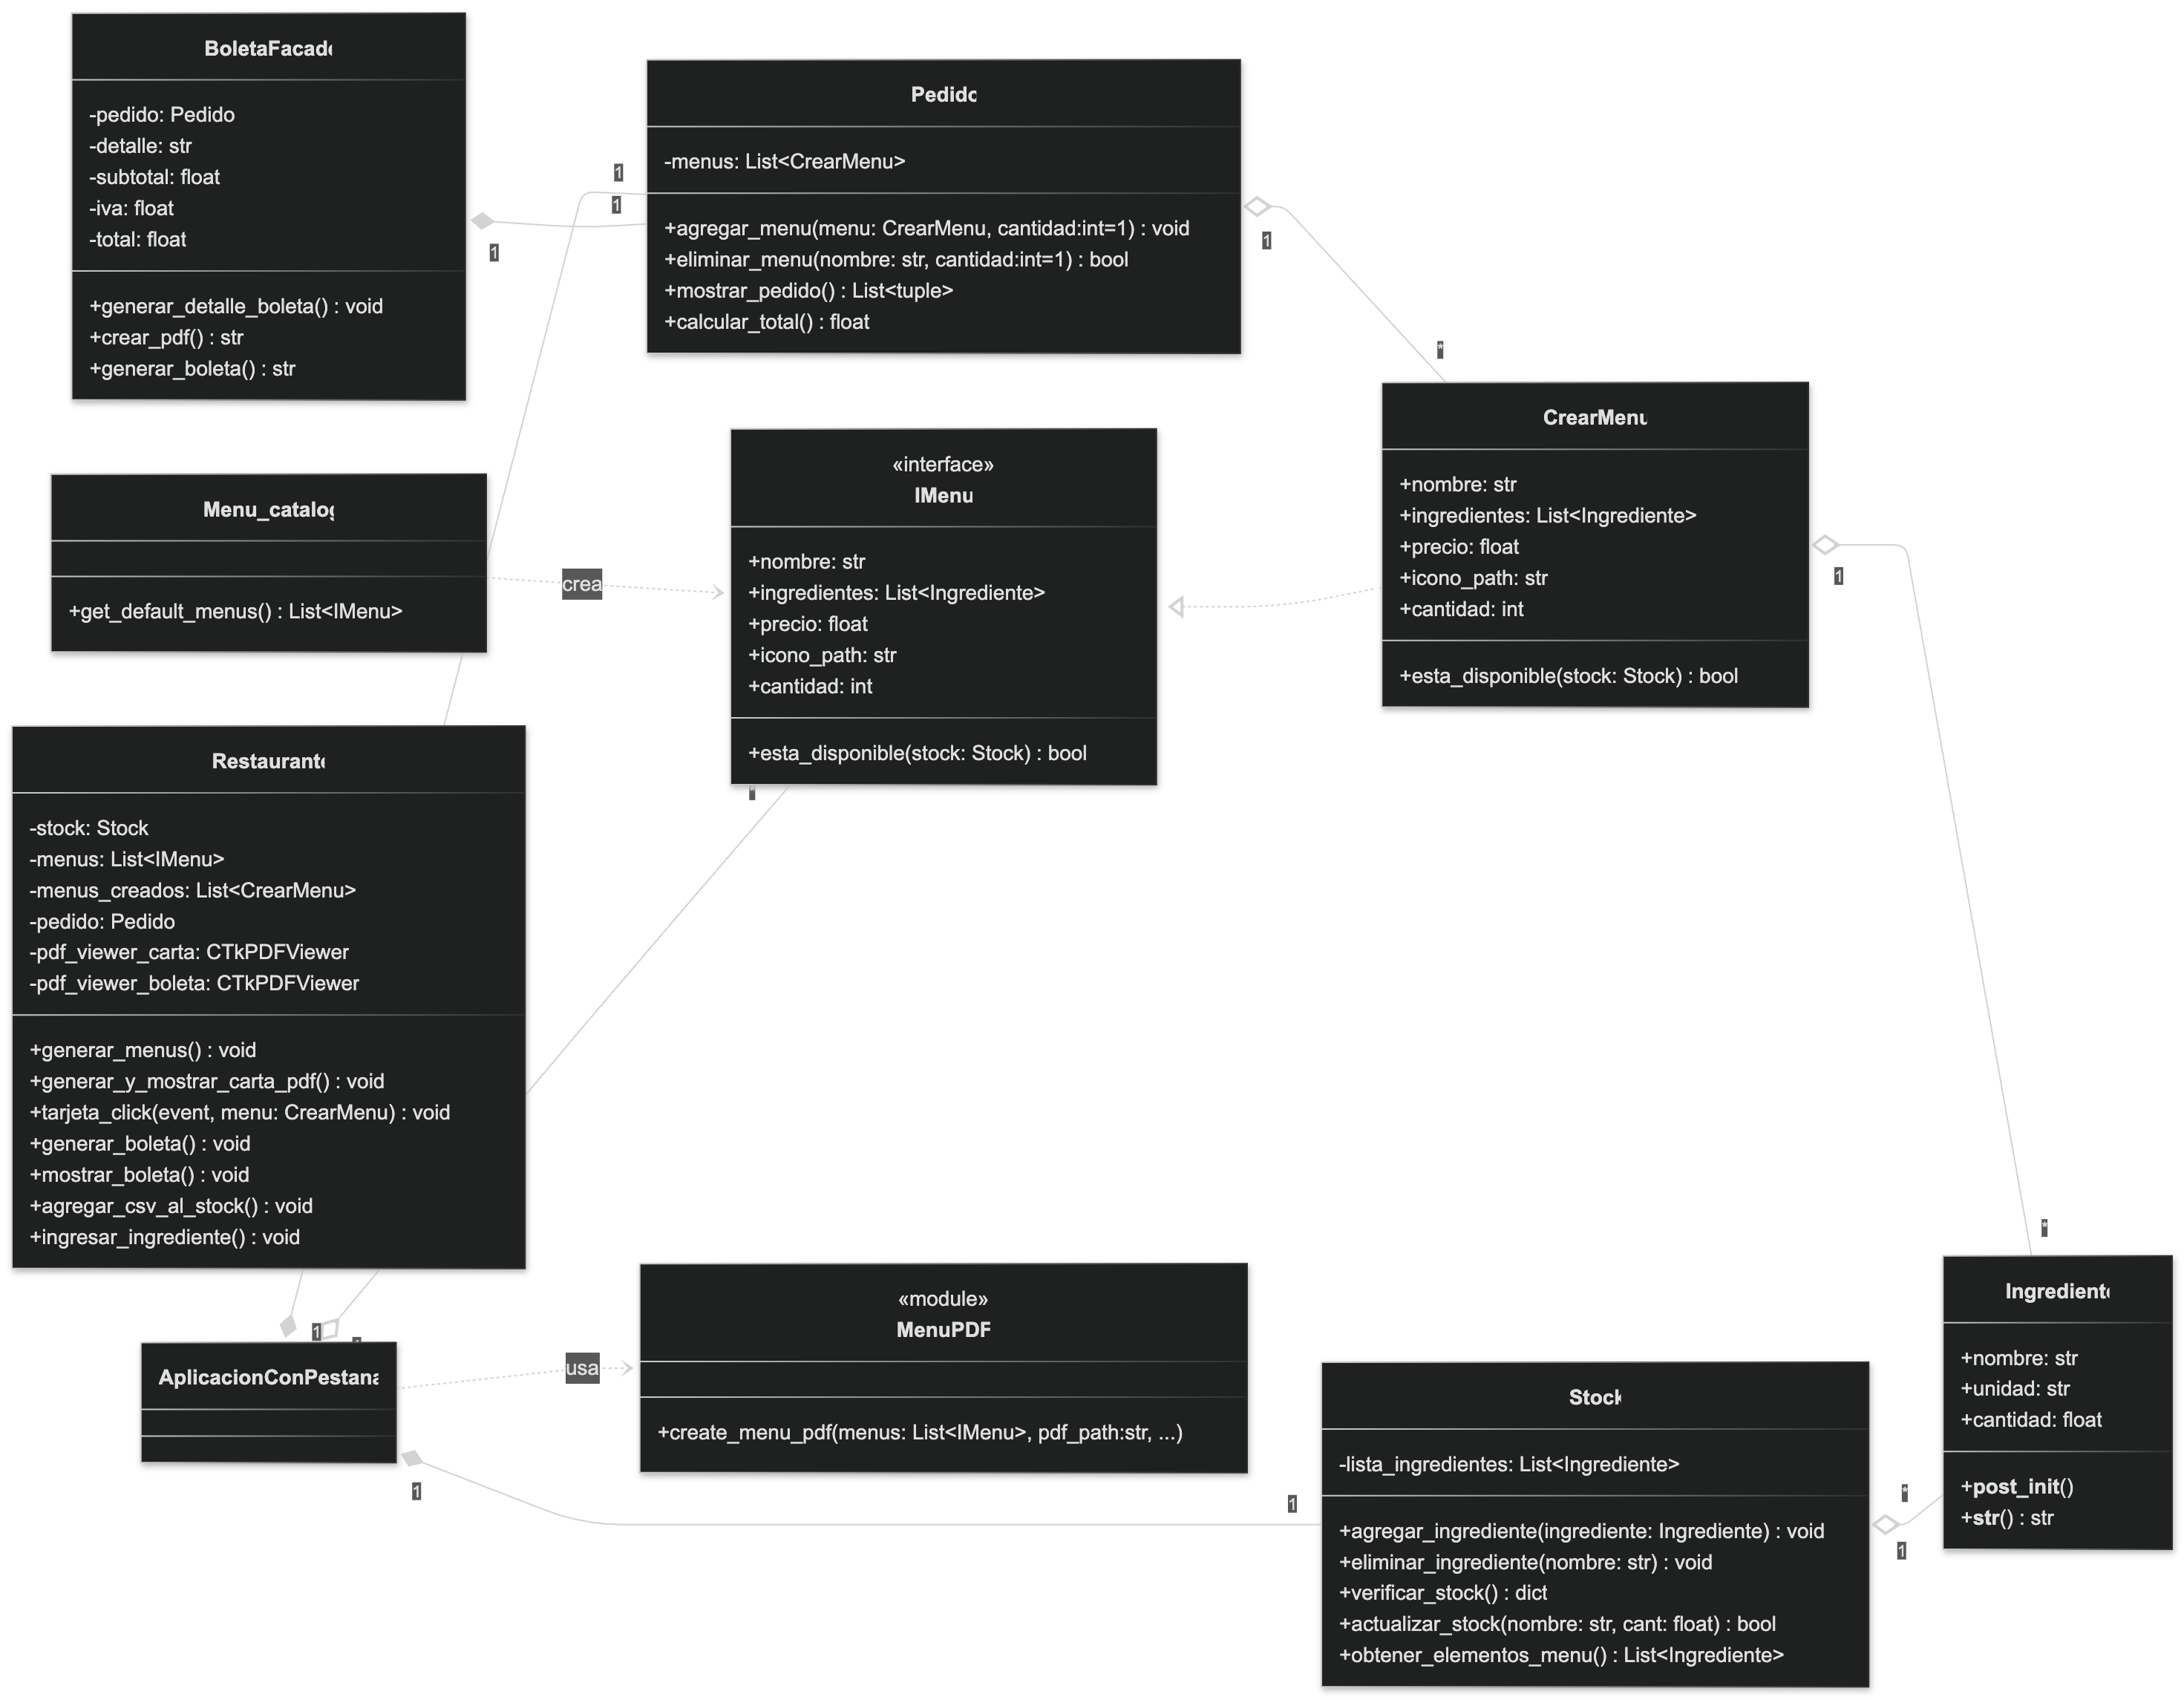
\includegraphics[width=\textwidth]{diagramaclases}
  \caption{Diagrama de clases del sistema}
  \label{fig:diagrama_clases}
\end{figure}

Primero, el usuario interactúa con la interfaz principal \texttt{AplicacionConPestanas}, que gestiona las funciones del sistema a través de la clase \texttt{Restaurant}. Desde ahí se pueden cargar ingredientes manualmente o desde un archivo CSV, actualizando el \texttt{Stock}, que mantiene la lista de \texttt{Ingrediente} y permite agregarlos, eliminarlos o ajustar sus cantidades.

Después, la aplicación genera los menús usando el catálogo base de \texttt{Menu\_catalog}. Cada \texttt{CrearMenu} revisa su disponibilidad con \texttt{esta\_disponible}, comparando los ingredientes necesarios con el \texttt{Stock}. Solo los menús con todos los ingredientes disponibles se incluyen en la carta, que se genera en PDF mediante \texttt{MenuPDF} y se muestra con \texttt{CTkPDFViewer}.

Cuando un cliente hace un pedido, \texttt{Pedido} guarda los menús seleccionados, controla cantidades y calcula subtotales y totales. Luego, \texttt{BoletaFacade} usa esta información para generar la boleta en PDF con detalle, subtotal, IVA y total, separando la lógica de generación de documentos de la interfaz.

En todo momento, el \texttt{Stock} es el centro del sistema: cualquier cambio en los ingredientes afecta directamente los menús disponibles, la carta y los pedidos, manteniendo todo actualizado y coherente.


\newpage

\section{Explicación de cada pestaña (paso a paso, con highlights de código)}

\subsection{Pestaña: Carga de ingredientes}
\textbf{Objetivo:} cargar CSV/Excel, normalizar columnas, previsualizar y subir al stock.

\paragraph{Flujo resumido}
\begin{enumerate}[leftmargin=*]
  \item Botón \textbf{Cargar CSV o Excel} (\texttt{cargar\_csv}) abre archivo, lo lee y genera cabeceras.
  \item Se muestra vista previa en un \texttt{Treeview} (\texttt{mostrar\_dataframe\_en\_tabla}).
  \item Botón \textbf{Agregar al Stock} (\texttt{agregar\_csv\_al\_stock}) valida unidad/cantidad y agrega al \texttt{Stock}.
\end{enumerate}

\begin{tcolorbox}[colback=yellow!6,colframe=yellow!50!black,title=Highlight de código — Carga (\texttt{cargar\_csv} y \texttt{agregar\_csv\_al\_stock})]
\lstset{style=pyclean}
\begin{lstlisting}
# Normaliza cabeceras y valida columnas requeridas
df = df.rename(columns={c: c.strip().lower() for c in df.columns})
requeridas = ('nombre', 'unidad', 'cantidad')
faltan = [c for c in requeridas if c not in df.columns]
if faltan:
    CTkMessagebox(title='Columnas Faltantes', message=..., icon='warning'); return

# Validación por fila antes de tocar el Stock
for _, row in df.iterrows():
    nombre = str(row['nombre']).strip(); unidad = str(row['unidad']).strip(); cantidad = row['cantidad']
    if unidad not in ("kg", "unid"):
        CTkMessagebox(title="Unidad inválida", message=..., icon="warning"); continue
    try: cantidad = float(cantidad)
    except: CTkMessagebox(title="Dato inválido", message=..., icon="warning"); continue
    if unidad == "unid": cantidad = int(cantidad)
    self.stock.agregar_ingrediente(Ingrediente(nombre, unidad, cantidad))
\end{lstlisting}
\textbf{¿Por qué este fragmento y qué hace?} Este bloque de código limpia y revisa los datos antes de guardarlos en el sistema. Así evita que entren datos incorrectos al Stock, lo que podría causar errores en las partes de Carta o Pedido.
\end{tcolorbox}
\newpage

\subsection{Pestaña: Stock}
\textbf{Objetivo:} alta/baja de ingredientes y generación de menús disponibles.

\paragraph{Flujo resumido}
\begin{enumerate}[leftmargin=*]
  \item Validaciones de nombre (solo letras/espacios), unidad y cantidad positiva.
  \item \textbf{Ingresar Ingrediente} llama a \texttt{Stock.agregar\_ingrediente}.
  \item \textbf{Eliminar Ingrediente} remueve por nombre.
  \item \textbf{Generar Menú} ejecuta \texttt{generar\_menus} (filtra por \texttt{esta\_disponible}).
\end{enumerate}

\begin{tcolorbox}[colback=green!6,colframe=green!60!black,title=Highlight de código — Stock (\texttt{agregar\_ingrediente})]
\lstset{style=pyclean}
\begin{lstlisting}
# Merge controlado por (nombre, unidad)
nombre_nuevo = ingrediente.nombre.strip().capitalize(); unidad_nueva = ingrediente.unidad
for ing in self._lista_ingredientes:
    if ing.nombre.capitalize() == nombre_nuevo and ing.unidad == unidad_nueva:
        ing.cantidad = float(ing.cantidad) + float(ingrediente.cantidad); return
    elif ing.nombre.capitalize() == nombre_nuevo and ing.unidad != unidad_nueva:
        CTkMessagebox(title="Error de unidad", message=... , icon="warning"); return
ingrediente.nombre = nombre_nuevo; self._lista_ingredientes.append(ingrediente)
\end{lstlisting}
\textbf{¿Por qué este fragmento y qué hace?} Evita duplicados incoherentes (mismo nombre, distinta unidad) y consolida cantidades; protege la integridad del stock.
\end{tcolorbox}
\newpage

\subsection{Pestaña: Pedido}
\textbf{Objetivo:} vender menús disponibles, descontar stock y calcular totales.

\paragraph{Flujo resumido}
\begin{enumerate}[leftmargin=*]
  \item Tarjetas clicables ejecutan \texttt{tarjeta\_click}.
  \item Se valida stock ingrediente por ingrediente; si no alcanza, se informa.
  \item Si alcanza: se descuenta del \texttt{Stock}, se agrega al \texttt{Pedido}, se actualiza UI y total.
\end{enumerate}

\begin{tcolorbox}[colback=red!6,colframe=red!60!black,title=Highlight de código — Pedido (\texttt{tarjeta\_click})]
\lstset{style=pyclean}
\begin{lstlisting}
# Núcleo de venta: validar y descontar
def tarjeta_click(self, event, menu):
    suficiente_stock = True if self.stock.lista_ingredientes else False
    for req in menu.ingredientes:
        for ing in self.stock.lista_ingredientes:
            if req.nombre == ing.nombre and float(ing.cantidad) < float(req.cantidad):
                suficiente_stock = False; break
        if not suficiente_stock: break
    if not suficiente_stock:
        CTkMessagebox(title="Stock Insuficiente", message=f"No hay suficientes para '{menu.nombre}'."); return
    # Descuento real
    for req in menu.ingredientes:
        for ing in self.stock.lista_ingredientes:
            if req.nombre == ing.nombre:
                nueva = float(ing.cantidad) - float(req.cantidad)
                ing.cantidad = int(nueva) if ing.unidad=='unid' else nueva
    self.pedido.agregar_menu(menu);
    self.actualizar_treeview_pedido();
    self.label_total.configure(text=f"Total: ${self.pedido.calcular_total():.2f}")
\end{lstlisting}
\textbf{¿Por qué este fragmento y qué hace?} Valida y descuenta el stock, respetando unidad de medida y sincronia Pedido/Stock con el treeview (tabla y total).
\end{tcolorbox}
\newpage

\subsection{Pestaña: Carta restaurante}
\textbf{Objetivo:} generar un PDF en tiempo real con menús disponibles.

\paragraph{Flujo resumido}
\begin{enumerate}[leftmargin=*]
  \item Botón \textbf{Generar Carta (PDF)} llama a \texttt{generar\_y\_mostrar\_carta\_pdf}.
  \item Filtra por \texttt{esta\_disponible}, exporta con \texttt{create\_menu\_pdf} y muestra con \texttt{CTkPDFViewer}.
\end{enumerate}

\begin{tcolorbox}[colback=purple!6,colframe=purple!60!black,title=Highlight de código — Carta (\texttt{generar\_y\_mostrar\_carta\_pdf})]
\lstset{style=pyclean}
\begin{lstlisting}
menus_para_pdf = [m for m in self.menus if m.esta_disponible(self.stock)]
if not menus_para_pdf:
    CTkMessagebox(title="Sin datos", message="No hay menús disponibles con el stock actual...", icon="warning"); return
abs_pdf = create_menu_pdf(
    menus=menus_para_pdf, pdf_path="carta.pdf",
    titulo_negocio="Restaurante", subtitulo="Carta (según stock)", moneda="$",
)
# Montaje seguro del visor
if self.pdf_viewer_carta is not None:
    self.pdf_viewer_carta.pack_forget(); self.pdf_viewer_carta.destroy(); self.pdf_viewer_carta=None
self.pdf_viewer_carta = CTkPDFViewer(self.pdf_frame_carta, file=abs_pdf)
self.pdf_viewer_carta.pack(expand=True, fill="both")
\end{lstlisting}
\textbf{¿Por qué este fragmento y qué hace?} Reusa la misma regla de disponibilidad que Pedido, y limpia la imagen anterior (Si es que existía) para evitar errores.
\end{tcolorbox}
\newpage

\subsection{Pestaña: Boleta}
\textbf{Objetivo:} emitir una boleta detallada (Subtotal, IVA, Total).

\paragraph{Flujo resumido}
\begin{enumerate}[leftmargin=*]
  \item \texttt{generar\_boleta} coordina \texttt{BoletaFacade}, reinicia el pedido y notifica.
  \item \texttt{mostrar\_boleta} renderiza el PDF si existe.
\end{enumerate}

\begin{tcolorbox}[colback=orange!6,colframe=orange!80!black,title=Highlight de código — Boleta (\texttt{generar\_boleta} y \texttt{mostrar\_boleta})]
\lstset{style=pyclean}
\begin{lstlisting}
# Coordinación desde la UI
if not self.pedido.menus:
    CTkMessagebox(title="Sin items", message="El pedido está vacío.", icon="warning"); return
facade = BoletaFacade(self.pedido)
facade.generar_boleta()  # calcula subtotal/IVA/total y crea boleta.pdf
self.pedido = Pedido(); self.actualizar_treeview_pedido(); self.label_total.configure(text="Total: $0.00")
CTkMessagebox(title="Boleta Generada", message="Ve a 'Boleta' y pulsa 'Mostrar Boleta'...")

 Visualización segura
def mostrar_boleta(self):
    pdf_path = os.path.abspath("boleta.pdf")
    if not os.path.exists(pdf_path):
        CTkMessagebox(title="Sin boleta", message="Primero genera boleta...", icon="warning"); return
    if self.pdf_viewer_boleta is not None:
        self.pdf_viewer_boleta.pack_forget(); self.pdf_viewer_boleta.destroy(); self.pdf_viewer_boleta=None
    self.pdf_viewer_boleta = CTkPDFViewer(self.pdf_frame_boleta, file=pdf_path)
    self.pdf_viewer_boleta.pack(expand=True, fill="both")
\end{lstlisting}
\textbf{¿Por qué este fragmento y qué hace?} Revisa si hay algo en el pedido; si está vacío, muestra un aviso y no sigue.  
Si hay menús, genera la boleta con \texttt{BoletaFacade}, que calcula subtotal, IVA y total, y crea el PDF.  
Luego deja todo limpio para la siguiente venta y avisa que la boleta fue generada.  
La parte de \texttt{mostrar\_boleta} se encarga de abrir el PDF dentro de la app de forma segura, reemplazando la imagen anterior si ya había una.
\end{tcolorbox}
\newpage

\section{Decisiones de diseño y justificación}
\begin{itemize}[leftmargin=*]
  \item \textbf{Encapsulación con propiedades}: \codehl{Stock.\_lista\_ingredientes} y \codehl{Pedido.\_menus} son privados para evitar mutaciones arbitrarias desde la UI. Se exponen \texttt{@property} de solo lectura y métodos controlados (agregar/eliminar).
  \item \textbf{\textit{Protocol} (\texttt{IMenu})}: permite intercambiar implementaciones de menús sin acoplar la UI, útil si mañana vienen menús dinámicos desde BD o API.
  \item \textbf{\textit{Dataclass} (\texttt{Ingrediente})}: menos código repetitivo y \textit{type hints} claros; \texttt{\_\_post\_init\_\_} fuerza cantidad a \texttt{float} para cálculos consistentes.
  \item \textbf{Unidades acotadas}: sólo “kg” y “unid” para simplificar validaciones y evitar combinaciones absurdas. Se mantuvo "kg" para mostrar el manejo de errores.
  \item \textbf{Normalización temprana}: nombres capitalizados y columnas en minúsculas. Para evitar errores a la hora de comparar variables.
  \item \textbf{UX explícita}: mensajes de error con \texttt{CTkMessagebox} en el punto donde el usuario toma acción.
\end{itemize}
\newpage

\section{Vínculo al repositorio}
Código fuente completo: \\ \href{https://github.com/notKechai/Programacion-II-Evaluacion-2}{https://github.com/notKechai/Programacion-II-Evaluacion-2}


\section{Cómo ejecutar}
\begin{enumerate}[leftmargin=*]
  \item Instale dependencias: \texttt{customtkinter}, \texttt{fpdf}, \texttt{Pillow}, \texttt{pandas}, \texttt{PyMuPDF}, etc.
  \item Ejecute \texttt{Restaurante.py}. Cargue un CSV/Excel o ingrese ingredientes manualmente.
  \item Genere menús, arme un pedido, emita boleta y/o exporte la carta en PDF.
\end{enumerate}

Las imágenes de iconos y el logo deben existir en las rutas indicadas. Ajuste nombres si es necesario.

\newpage

\section{Conclusión}
El sistema desarrollado cumple con los objetivos planteados, ofreciendo una herramienta práctica y confiable para la administración de restaurantes pequeños o medianos. Permite cargar ingredientes de manera segura, mantener el stock consistente, generar la carta y los pedidos de forma sincronizada, y emitir boletas en PDF con todos los cálculos correspondientes.

En resumen, el proyecto demuestra cómo la programación orientada a objetos y un diseño modular permiten crear soluciones escalables y eficientes para la gestión de restaurantes, mejorando y facilitando futuras extensiones del sistema.

\end{document}